\documentclass{article}
\usepackage{fullpage,subfigure,fancyhdr}
\usepackage[pdftex]{color}
\usepackage{wrapfig}
\usepackage{textcomp}
\usepackage{verbatim}
\usepackage{times}
\usepackage{amsfonts,amsmath,amssymb,amsthm}
\usepackage{textcomp}
\usepackage{url}
\usepackage{mdwlist}
\usepackage{subfigure}
\usepackage{sidecap}
\usepackage{wrapfig}
\usepackage{xspace}
\usepackage{algorithm,algorithmic}
\usepackage[pdftex]{graphicx}
\usepackage[colorlinks=true,pagebackref,linkcolor=magenta]{hyperref}
\usepackage[sort&compress,comma,round,numbers]{natbib}
\usepackage{pict2e}
\usepackage[nottoc,numbib]{tocbibind}
\usepackage{paralist}
\usepackage{multicol}
\usepackage{lettrine}
\usepackage{lineno}
% \usepackage{trackchanges}
% \usepackage{mcode}

\usepackage{helvet}
\renewcommand{\familydefault}{\sfdefault}
\definecolor{MyGray}{rgb}{0.7,0.7,0.7}

% \numberwithin{figure}{section}
% \numberwithin{table}{section}
% \numberwithin{algorithm}{section}


%%%%% COLOR STUFF %%%%%%%%%%
\newcommand{\db}[1]{{\color{dark_blue}{#1}}}
\newcommand{\bb}[1]{{\textbf{\db{#1}}}}

\definecolor{MyPlum}{rgb}{0.3,0,0.3}
\definecolor{MyOrange}{rgb}{1,0.5,0}
\definecolor{deep_blue}{rgb}{0,.2,.5}
\definecolor{dark_blue}{rgb}{0,.15,.5}

\newcommand{\marta}[1]{{\color{red}{\it marta: #1}}}
\newcommand{\youngser}[1]{{\color{green}{\it youngser: #1}}}
\newcommand{\brett}[1]{{\color{blue}{\it brett says: #1}}}
\newcommand{\jovo}[1]{{\color{magenta}{\it JoVo: #1}}}
\newcommand{\rb}[1]{{\color{red}{\it rb: #1}}}
\newcommand{\bro}[1]{{\color{blue}{\it youngser: #1}}}
\newcommand{\agastya}[1]{{\color{red}{\it agastya: #1}}}
\providecommand{\tg}[1]{\textcolor{green}{#1}}
\providecommand{\tb}[1]{\textcolor{blue}{#1}}
\providecommand{\tr}[1]{\textcolor{red}{#1}}
\providecommand{\tk}[1]{\textcolor{black}{#1}}
\providecommand{\twhite}[1]{\textcolor{white}{#1}}


%%%%%%%%% MATH OPERATORS %%%%%%%%%%%%
\providecommand{\ve}[1]{\boldsymbol{#1}}
\providecommand{\ma}[1]{\boldsymbol{#1}}
\providecommand{\norm}[1]{\left \lVert#1 \right  \rVert}
\providecommand{\deter}[1]{\lvert #1 \rvert}
\providecommand{\abs}[1]{\left \lvert #1 \right \rvert}
\providecommand{\mat}[1]{\left[ #1 \right]}
\newcommand{\trans}[1]{{#1}^{\ensuremath{\mathsf{T}}}}           % transpose
\newcommand{\transpose}[1]{{#1}^{\ensuremath{\mathsf{T}}}}           % transpose
\newcommand{\argmax}{\operatornamewithlimits{argmax}}
\newcommand{\argmin}{\operatornamewithlimits{argmin}}
\newcommand{\T}{^{\ensuremath{\mathsf{T}}}}           % transpose
\newcommand{\from}{{\ensuremath{\colon}}}           % :
\newcommand{\trace}[1]{{\ensuremath{\operatorname{tr}\!\left(#1\right)}}}           % :

\providecommand{\ms}[1]{\mathsf{#1}}
\providecommand{\mc}[1]{\mathcal{#1}}
\providecommand{\mb}[1]{\boldsymbol{#1}}
\providecommand{\mbb}[1]{\mathbb{#1}}
\providecommand{\mv}[1]{\vec{#1}}
\providecommand{\mh}[1]{\hat{#1}}
\providecommand{\wh}[1]{\widehat{#1}}
\providecommand{\mhv}[1]{\mh{\mv{#1}}}
\providecommand{\mvh}[1]{\mv{\mh{#1}}}
\providecommand{\mt}[1]{\widetilde{#1}}
\providecommand{\mhc}[1]{\hat{\mathcal{#1}}}
\providecommand{\mbc}[1]{\mb{\mathcal{#1}}}
\providecommand{\mvc}[1]{\mv{\mathcal{#1}}}
\providecommand{\mtc}[1]{\widetilde{\mathcal{#1}}}
\providecommand{\mth}[1]{\mt{\mh{#1}}}
\providecommand{\mht}[1]{\mh{\mt{#1}}}
\providecommand{\mhb}[1]{\hat{\boldsymbol{#1}}}
\providecommand{\whb}[1]{\widehat{\boldsymbol{#1}}}
\providecommand{\mvb}[1]{\vec{\boldsymbol{#1}}}
\providecommand{\mtb}[1]{\widetilde{\boldsymbol{#1}}}
\providecommand{\mbt}[1]{\widetilde{\boldsymbol{#1}}}
\providecommand{\mvc}[1]{\vec{\mathcal{#1}}}
% \newcommand{\D}[2]{\frac{\partial #1}{\partial #2}}
\newcommand{\dd}[2]{\frac{\partial ^2 #1}{\partial #2 ^2}}
\newcommand{\DDD}[3]{\frac{\partial ^2 #1}{\partial #2 \partial #3}}
\newcommand{\Di}[2]{\frac{\partial ^i #1}{\partial #2 ^i}}



%%%%%%%%%% SECTIONS & STUFF %%%%%%%%%%%%%

\newtheorem{Rem}{Remark}%[section]
\newtheorem{Alg}{Algorithm}%[section]
\newtheorem{thm}{Theorem}
\newtheorem{lem}{Lemma}
\newtheorem{Thm}{Theorem}[section]
\newtheorem{Lem}{Lemma}%[section]
\newtheorem{defi}{Definition}
\newtheorem{Def}{Definition}[section]
\newtheorem{prop}{Proposition}
\newtheorem{coro}[thm]{Corollary}
\newtheorem{claim}{Claim}
\newtheorem{conj}{Conjecture}
\newtheorem{question}{Question}
\newtheorem{rem}{Remark}%[section]
\newtheorem{cor}[lem]{Corollary}
\newtheorem{model}{Model}

\newcommand{\bla}{\begin{block}}
\newcommand{\blb}{\end{block}}

\newcommand{\defa}{\begin{defi}}
\newcommand{\defb}{\end{defi}}
\newcommand{\theHalgorithm}{\arabic{algorithm}}

\newcommand{\thma}{\begin{thm}}
\newcommand{\thmb}{\end{thm}}

\newcommand{\mata}{\begin{bmatrix}}
\newcommand{\matb}{\end{bmatrix}}

\floatname{algorithm}{Procedure}
\renewcommand{\algorithmicrequire}{\textbf{Input:}}
\renewcommand{\algorithmicensure}{\textbf{Output:}}
\floatname{algorithm}{Pseudocode}



%%%%%% section stuff %%%%%%%%%%
\renewcommand{\thesection}{\Roman{section}}   % set the section counter to Alpha
\renewcommand{\thesubsection}{\Roman{section}.\Alph{subsection}}   % set the subsection counter to alpha
% \renewcommand{\thesubsubsection}{\Alph{section}.\arabic{subsection}(\arabic{subsubsection})}   % set the subsection counter to alpha
% 
% 
\makeatletter
% \def\subsize{\@setsize\subsize{8pt}\xipt\@xipt}
 \def\section{\@startsection {section}{1}{\z@}{5pt}{9pt}{\Large\bf\db}}
 \def\subsection{\@startsection {subsection}{2}{\z@}{10pt}{4pt}{\large\bf\db}}
 \def\subsubsection{\@startsection {subsubsection}{2}{\z@}{10pt}{4pt}{\bf\db}}
% \def\subs{\@startsection {subsubsection}{2}{0pt}{5pt}{0pt}{ \subsize\bf\db}}
\def\paragraph{\@startsection {paragraph}{2}{\z@}{10pt}{4pt}{\bf\db}}
% \def\subparagraph{\@startsection 


\newcommand{\para}[1]{\vspace{3pt}\noindent{{\fontsize{11pt}{1em} \bf #1}}}
\newcommand{\subpara}[1]{\vspace{3pt}\noindent{{\fontsize{11pt}{1em} \bf \emph{#1}}}}
\newcommand{\subsubpara}[1]{\vspace{3pt}\noindent{{\fontsize{10pt}{1em} \emph{#1}}}}


%%%%%% SHORT HAND %%%%%%%%%%
\renewcommand{\refname}{References and Notes}

\newcommand{\jv}{Joshua Vogelstein}
\newcommand{\jhu}{Johns Hopkins University}
\newcommand{\website}{http://jovo.me/}
\newcommand{\email}{jovo@jhu.edu}

\newcommand{\Vr}{V_{reset}}
\newcommand{\Vl}{V_{leat}}
\newcommand{\eqdef}{\overset{\triangle}{=}}
\newcommand{\grad}{\nabla}
\newcommand{\Hess}{\nabla\nabla}
\newcommand{\defn}{\overset{\triangle}{=}}

\newcommand{\iid}{\overset{iid}{\sim}}
\newcommand{\knn}{$k$NN}

\newcommand{\elegans}{\emph{C. elegans} }

\newcommand{\Lik}{\mathcal{L}}
\newcommand{\Cae}{[\widehat{\text{Ca}}^{2+}]}
\newcommand{\Cav}{\ve{C}}%[\ve{\text{Ca}}^{2+}]}
\newcommand{\sml}{\sqrt{\ma{\lambda}}}
\newcommand{\ml}{\ma{\lambda}}
\newcommand{\nw}{\widehat{n}}
\newcommand{\nv}{\vec{n}}
\newcommand{\Ae}{\widehat{A}}
\newcommand{\te}{\widehat{\tau}}
\newcommand{\maxn}{\max_{\ve{n}: n_t \geq 0}}
% \newcommand{\V}{\text{Var}}

\newcommand{\PmcP}{P \in \mc{P}}
\newcommand{\mP}{\mathbb{P}}

% \newcommand{\dvs}{\dot{\bs}_t}
% \newcommand{\dvw}{\dot{\bw}_t}
% \newcommand{\dvx}{\dot{\bx}_t}
% \newcommand{\dvy}{\dot{\by}_t}

\newcommand{\ft}{f_{\ve{\thet}}}
\newcommand{\gt}{g_{\ve{\thet}}}
\newcommand{\hht}{h_{\thetn}}

\newcommand{\Real}{\mathbb{R}}



\newcommand{\wconv}{\overset{i.p.}{\rightarrow}}
\newcommand{\sconv}{\overset{i.p.}{\rightarrow}}
\newcommand{\conv}{\rightarrow}
\newcommand{\pconv}{\overset{p}{\conv}}
\newcommand{\mcE}{\mathcal{E}}
\newcommand{\mcT}{\mathcal{T}}
\newcommand{\mcG}{\mathcal{G}}
\newcommand{\mcM}{\mathcal{M}}
\newcommand{\mcL}{\mathcal{L}}
\newcommand{\hatmcE}{\widehat{\mcE}}
\newcommand{\hatp}{\widehat{p}}
\newcommand{\hatP}{\widehat{P}}
\newcommand{\hatQ}{\widehat{Q}}
\newcommand{\hatL}{\widehat{L}}
\newcommand{\mhP}{\widehat{\PP}}
\newcommand{\tildeA}{\widetilde{A}}
\newcommand{\defeq}{\overset{\triangle}{=}}


\DeclareMathOperator{\Pmat}{\mathbf{P}}
\DeclareMathOperator{\veta}{\mathbf{\mb{v}}}
\DeclareMathOperator*{\minimize}{\mathrm{minimize}}
\DeclareMathOperator*{\maximize}{\mathrm{maximize}}
% \DeclareMathOperator*{\mb{v}mod}{\mathbf{\mb{v}}}


%%%%%%% LATIN LETTERS


\newcommand{\bA}{\mb{A}}
\newcommand{\bB}{\mb{B}}
\newcommand{\bI}{\mb{I}}
\newcommand{\bP}{\mb{P}}
\newcommand{\bS}{\mb{S}}
\newcommand{\bU}{\mb{U}}
\newcommand{\bV}{\mb{V}}
\newcommand{\bW}{\mb{W}}
\newcommand{\bX}{\mb{X}}
\newcommand{\bY}{\mb{Y}}

\newcommand{\ba}{\mb{a}}
\renewcommand{\ba}{\mb{b}}
\newcommand{\bp}{\mb{p}}
\newcommand{\bs}{\mb{s}}
\newcommand{\bu}{\mb{u}}
\newcommand{\bv}{\mb{v}}
\newcommand{\bw}{\mb{w}}
\newcommand{\bx}{\mb{x}}
\newcommand{\by}{\mb{y}}


\newcommand{\Aa}{\mathbb{A}}
\newcommand{\BB}{\mathbb{B}}
\newcommand{\CC}{\mathbb{C}}         
\newcommand{\DD}{\mathbb{D}}         
\newcommand{\EE}{\mathbb{E}}           % expected value
\newcommand{\FF}{\mathbb{F}}         
\newcommand{\GG}{\mathbb{G}}
\newcommand{\HH}{\mathbb{H}}         
\newcommand{\II}{\mathbb{I}}           % indicator function
\newcommand{\LL}{\mathbb{L}}
\newcommand{\MM}{\mathbb{M}}
\newcommand{\NN}{\mathbb{N}}
\newcommand{\PP}{\mathbb{P}}         
\newcommand{\QQ}{\mathbb{Q}}           
\newcommand{\SSS}{\mathbb{S}}           
\newcommand{\VV}{\mathbb{V}}
\newcommand{\WW}{\mathbb{W}}         
\newcommand{\XX}{\mathbb{X}}         
\newcommand{\YY}{\mathbb{Y}}
\newcommand{\ZZ}{\mathbb{Z}}         




\newcommand{\Qs}{Q}
\newcommand{\mcS}{\mc{S}}
\newcommand{\mcU}{\mc{U}}

\newcommand{\mbd}{\mb{d}}
\newcommand{\mbD}{\mb{D}}
\newcommand{\mbx}{\mb{x}}
\newcommand{\mbX}{\mb{X}}
\newcommand{\mby}{\mb{y}}
\newcommand{\mbY}{\mb{Y}}

\newcommand{\mtbd}{\mtb{d}}
\newcommand{\mtbD}{\mtb{D}}
\newcommand{\mtbx}{\mtb{x}}
\newcommand{\mtbX}{\mtb{X}}
\newcommand{\mtby}{\mtb{y}}
\newcommand{\mtbY}{\mtb{Y}}



\DeclareMathOperator{\Ri}{\mathbf{\R}^{-1}}
\DeclareMathOperator{\A}{A}
\DeclareMathOperator{\W}{\mathbf{W}}
\DeclareMathOperator{\V}{\mathbf{V}}
\DeclareMathOperator{\U}{\mathbf{U}}
\DeclareMathOperator{\C}{\mathbf{C}}
\DeclareMathOperator{\uvec}{\mathbf{u}}
\DeclareMathOperator{\D}{\mathbf{D}}
\DeclareMathOperator{\Q}{\mathbf{Q}}
\DeclareMathOperator{\R}{R} %\mathbf{P}}
\DeclareMathOperator{\Y}{\mathbf{Y}}
\DeclareMathOperator{\B}{\mathbf{B}}
\DeclareMathOperator{\Hmat}{\mathbf{H}}
\DeclareMathOperator{\Gmat}{\mathbf{G}}
\DeclareMathOperator{\X}{\mathbf{X}}
\DeclareMathOperator{\Cmat}{C} %\mathbf{L}}\providecommand{\ms}[1]{\mathsf{#1}}

\DeclareMathOperator*{\Ymod}{\mathbf{\Y}}
\DeclareMathOperator*{\Bmod}{\mathbf{B}}
\DeclareMathOperator*{\Hmod}{\mathbf{H}}
\DeclareMathOperator*{\Lmod}{\mathbf{L}}
\DeclareMathOperator*{\Xmod}{\mathbf{\X}}


%%% THETA %%%%

\newcommand{\bth}{\ve{\theta}}
\newcommand{\hth}{\mh{\theta}}
\newcommand{\htth}{\mh{\theta}}
\newcommand{\bhth}{\mh{\ve{\theta}}}
\newcommand{\thetn}{\ve{\theta}}
\newcommand{\thet}{\thetn}
\newcommand{\theth}{\widehat{\ve{\theta}}}
\newcommand{\theto}{\ve{\theta}'}
\newcommand{\wht}{\widehat{\thet}}
\newcommand{\wtt}{\widetilde{\thet}}
\newcommand{\vth}{\ve{\thet}}
\newcommand{\vTh}{\ve{\Theta}}
\newcommand{\hvth}{\widehat{\ve{\thet}}}
\newcommand{\bTh}{\ve{\Theta}}
\newcommand{\hbth}{\widehat{\thet}}
\newcommand{\tbth}{\tilde{\bth}}



% \newcommand{\p}{P_{\bth}}
\newcommand{\pold}{P_{\bth'}}
\newcommand{\pk}{P_{\widehat{\ve{\theta}}^{(k)}}}
\newcommand{\pT}{P_{\thetn_{Tr}}} %\thetn_T
\newcommand{\pO}{P_{\thetn_o}} %\thetn_o
% \newcommand{\Q}{Q(\thetn,\theto)}
% \newcommand{\m}{m^{\ast}}
% \newcommand{\q}{q(\ve{H}_t)}
\newcommand{\Ca}{[\text{Ca}^{2+}]}


%%%%%% GREEK LETTERS

\newcommand{\del}{\delta}
\newcommand{\sig}{\sigma}
\newcommand{\lam}{\lambda}
\newcommand{\gam}{\gamma}
\newcommand{\eps}{\varepsilon}

\newcommand{\Del}{\Delta}
\newcommand{\Sig}{\Sigma}
\newcommand{\Lam}{\Lambda}
\newcommand{\Gam}{\Gamma}

\newcommand{\bSig}{\ve{\Sigma}}
\newcommand{\bOm}{\ve{\Omega}}
\newcommand{\bLam}{\ve{\Lambda}}
\newcommand{\bPhi}{\ve{\Phi}}
\newcommand{\bPsi}{\ve{\Psi}}

\newcommand{\bmu}{\ve{\mu}}
\newcommand{\bal}{\ve{\alpha}}
\newcommand{\bpi}{\ve{\pi}}
\newcommand{\bkap}{\ve{\kappa}}
\newcommand{\bdel}{\ve{\delta}}
\newcommand{\bphi}{\ve{\phi}}
\newcommand{\bpsi}{\ve{\psi}}



\DeclareMathOperator{\Delti}{\mathbf{\Delta}^{-1}}
\DeclareMathOperator{\Delt}{Q} %\mathbf{\Delta}}
% \DeclareMathOperator{\Gam}{\mathbf{\Gamma}}
\DeclareMathOperator{\Gami}{\mathbf{\Gamma}^{-1}}
\DeclareMathOperator{\Sigb}{\mathbf{\Sigma}}






%%%%%%%%%%% ALGORITHM NAMES %%%%%%%%%%%%%

\newcommand{\FAQ}{\texttt{FAQ} }

\providecommand{\sct}[1]{{\sc \texttt{#1}}}
\newcommand{\msl}{{\sc Idt}}

\newcommand{\Svd}{\sct{Svd}}
\newcommand{\Pca}{\sct{Pca}}
\newcommand{\Fld}{\sct{Fld}}
\newcommand{\Lda}{\sct{Lda}}
\newcommand{\eig}{\sct{eig}}
\newcommand{\qr}{\sct{qr}}
\newcommand{\Lol}{\sct{Lol}}
\newcommand{\Lal}{\sct{Lal}}
\newcommand{\Lrl}{\sct{Lrl}}
\newcommand{\Lfl}{\sct{Lfl}}





\title{\vspace{-50pt}
% Reliable and Reproducible Brain-Based Measures for Candidate Biomarker Discovery from Big Data
% Optimal Discovery Science from Big Brain-Imaging Data via Reliability and Reproducibility  
\db{Optimal Design for Discovery Science (aka Unspecified Tasks) via Maximizing Discriminability: \\ Applications in Neuroimaging}
}
\author{Shangsi Wang, Zhi Yang, Xi-Nian Zuo, Michael Milham, Cameron Craddock,  \\ 
Greg Kiar, William Gray Roncal, Eric Bridgeford,
Consortium for Reliability and Reproducibility, \\ Carey E.~Priebe, Joshua T. Vogelstein}


\begin{document}

\maketitle

\section{Introduction}

The data age is enabling us as a society to answer both age old questions and brand new ones.  Fundamentally, to obtain quantitative answers to any inquiry requires making two decisions: (i) ``how should the data be collected?'', and (ii) ``how should the data be processed?''  Optimally addressing experimental design decisions can yield dramatic improvements in both the financial and inferential costs \cite{?}.  When the downstream inference task is known, a priori, the theory of experimental design tells us how to proceed \cite{Fisher1935}. 
% 
% Historically, however, much of the work has focused on designing  experiments with a specific hypothesis testing or estimation problem in mind \cite{Winer1965}.  In more recent times
Recently, across industry, governmental, and academic settings, certain datasets become benchmark or reference datasets.  Such datasets can then be used for a wide variety of different inferential problems. For example, the Sloan Digital Sky Survey (SDSS) data has been used to discover new quasars \cite{?}, and the human genome project data has revealed genetic insights into a many different diseases \cite{?}.  Collecting and processing these datasets requires massive institutional investments, and choices related to questions (i) and (ii) above have dramatic effects on all subsequent analyses.  Therefore, a theoretical framework to enable investigators to select from a set of possible design decisions using pilot data could reap great rewards.

The goal of such a framework would be to enable data set construction to be optimized for \emph{any} subsequent downstream inference task, including all those currently not yet even conceived \cite{Stanford2006}.  This is not possible, because different inference tasks have different sources of information.  
Instead, however, we can show that one can choose from amongst a set of alternatives to maximize a lower bound on all subsequent inference tasks.  
% 
Both recent and historical work in a discipline of study called ``Generalizability Theory'' has related goals. More specifically, it aims to analyze and quantify the various sources of error.  Intra-class correlation (ICC) \cite{Shroud1979} and Kendall's tau \cite{Kendall1938} are parametric and non-parametric methods, respectively, for evaluating the ``reliability'' of a particular univariate statistic (such as magnitude or direction).  More recently, I2C2 was proposed \cite{Shou2013} as a multivariate extension to ICC.   These methods, while quite powerful, also have certain limitations.  For example, ICC and Kendell's tau only operate on univariate data.  The motivating example for this work, however, is high-dimensional neuroimaging data.  The high-dimensional generalization of ICC, I2C2, makes certain parametric assumptions, and therefore is inappropriate in certain settings of interest, such as sparsity.  
% 
Moreover, we are not interested in quantifying the relative sources of error explicitly, rather, we have supervised learning problem; we desire to optimize performance on unknown tasks.  

To this end,  we have developed a  formal definition of discriminability, 
a non-parametric statistical property of a joint distribution in a hierarchical model, 
to reflect the trade-off across within and between entity variance.  
We prove that discriminability, provides a lower bound on predictive accuracy for any downstream inference task, even if we have never seen the covariates to predict.
% 
We then derive an estimator of discriminability, and derive our estimator's asymptotic distribution, demonstrating that it is unbiased. 
Numerical simulations demonstrate the utility of our discriminability estimator in a variety of settings.  Finally, we apply our approach to choose amongst a set of choices one must make when designing a neuroimaging study to specifically study connectomics.  We start by finding the maximally discriminable threshold for converting correlation matrices (sometimes called functional connectomes), into binary edge lists (or graphs).  Indeed, consistent with out theoretical and simulated results, maximizing the discriminability of our datasets also maximizes performance on a suite of different downstream inference tasks.  We then ask about a series of pre-processing steps: should one motion correct or not, and should one implement global signal regression or not, etc. We find the maximally discriminable strategy amongst a combinatorial set of options.  Moreover, the pre-processing strategy that maximizes discriminability also maximizes predictive accuracy on a suite of tests.  Finally, we apply our method to determine which dataset is more discriminable by comparing multiple different datasets.  We conclude that a particular dataset is more discriminable than the others, and that predictive accuracy from that dataset is improved relative to the others. 

Thus, in total, our discriminability analysis is a powerful tool for making decisions about how to collect and analyze datasets designed for discovery science.  We expect this method to be useful in a wide variety of applications, and therefore have made all the code open source and available from \url{http://neurodata.io}.


\section{Results}



\subsection{Theory}

\subsubsection{Definition of Discriminability}

\subsubsection{Optimizing discriminability Optimizes Bound on Performance for Any Task}


a useful definition of discriminability (R)

\begin{thm}
discriminability bounds predictive accuracy
\end{thm}


\subsubsection{Estimator/Test Statistic}

\begin{itemize}
\item an estimator of R, called Rhat

\item proof that our estimator is unbiased (in a model free setting), 
$E(Rhat)=R$.

\item proof that our estimator asymptotically converges to truth (in a model free setting), $\mh{R}_n \conv R$
\end{itemize}


\subsection{Simulations}

\subsubsection{}


\subsection{Connectome Applications}

\subsubsection{optimal reliablity yields optimal predictive accuracy}


\subsubsection{best pipeline = product of marginals}

\subsubsection{thresholding vs. binning ranks}

\subsubsection{which atlas/resolution}


\subsubsection{DTI vs. fMRI}










\section{Discussion}

\para{Summary}


\para{Recommendations}


\begin{itemize}
\item Prior to embarking on any new large experimental data collection and analysis, we recommend generating a pilot dataset amenable to discriminability analysis.
\item Upon designing a new experiment or analysis, we recommend discriminability, as defined in Eq.~\eqref{eq:R}, as the criterion upon which to optimize decisions.
\item Because data analytics now have a large number of software dependencies, to maximize discriminability of analytics workstreams, we recommend packaging all necessary software into portable deployable systems, such as vagrant
\item For Human multimodal MRI connectomics, assuming the hardware system and scanner are sufficiently similar to those studies in this manuscript, we recommend using the reference pipelines  
\end{itemize}


\begin{itemize}
\item Upon designing a new experiment or analysis, we recommend discriminability, as defined in Eq.~\eqref{eq:R}, as the criterion upon which to optimize decisions.
\item Because data analytics now have a large number of software dependencies, to maximize discriminability of analytics workstreams, we recommend packaging all necessary software into portable deployable systems, such as vagrant
\end{itemize}


\para{Next Steps}


% \input{intro}
% \input{simulations}
% \input{flow}
% \input{setting}
% \input{logic}
% \input{main}
% \input{setup}
% \input{gRAICAR}



\appendix



\section{Introduction}

In many problems arising in the data science, data preprocessing is the first step toward statistical inference. In this era, data usually comes with high dimensionality and in complicated forms which make directly working with raw data almost impossible. Therefore, necessary preprocessing must be performed to prepare the data ready for subsequent inference task. However, this crucial first step is sometimes done in an arbitrary or subjective fashion which lacks proper guidance and theoretical justification. In our current work, we investigate the relationship between data preprocessing and supervised learning. In particular, we propose that data preprocessing should be done to maximize discriminability of processed data. We demonstate theoretically and with real data experiments that under supervised learning setting this approach produces data with small prediction error.\\
\\
Reliability refers to the overall consistency of a measure. For example, if a subject is measured twice under the same conditions, two measures should be close to each other given the measure is discriminable. The same spirit can be applied to data preprocessing. Good data preprocessing method should be discriminable which means the processed data should have samples from the same subject close to each other. Actually, our analysis reveals that optimal data preprocessing is achieved when the discriminability of processed data is maximized. In order to compare and select among preprocessing methods, we first need to be able to measure the discriminability of processed data. \\
\\
Many successful attempts have been made toward measuring discriminability. Previous works include but not limit to Cohen's Kappa, Intraclass Correlation Coefficient (ICC), Bland Altman Test and Image intraclass correlation coefficient (I2C2). The key limitation the first three measure have is that they can only measure discriminability of one-dimensional data, which makes them not appropriate to apply in multidimensional data preprocessing circumstances. I2C2 is designed to capture signal-to-noise ratio of high dimensional data. However, I2C2 assumes data has additive noise and lies in Euclidean space equiped with $L_2$ norm. These assumptions make it hard to generalize and apply for real data. To overcome the disadvantages of previous measure, we propose to use mean normalized rank (MNR) as a new measure of discriminability. \\
\\
Let us first introduce some notations and the definition of normalized rank. Suppose there are $n$ subjects and each subject is measured $s$ times. Denote $O_{ij}$, for $1\leq i \leq n$, $1\leq j \leq s$ the $j$th observation on subject $i$. The normalized rank $R_{ijk}$, $k\neq j$ counts the number of observations from other subjects are closer to observation $O_{ij}$ compared to $O_{ik}$, and the count is then normalized by dividing the total number of observations from other subjects which is $(n-1)s$. That is,
\[R_{ijk} := \frac{\sum\limits_{p=1,p\neq i}^{n} \sum\limits_{q=1}^{s} I\{\|O_{ij}-O_{pq}\| < \|O_{ij}-O_{ik}\| \} }{(n-1)s}\]
 The normalized rank $R_{ijk}$ can be also understood as the rank of distance between $O_{ij}$ and $O_{ik}$, among the distances between observations of other subjects and $O_{ij}$, but the rank is rescaled to make sure it lies between 0 and 1. The definition of $R_{ijk}$ above can be easily generalized to metric space by replacing the norm $\|\cdot-\cdot\|$ with ditance $d(\cdot,\cdot)$. There are two things to notice. First, when computing the rank of $\|O_{ij}-O_{ik}\|$, the distances between other observations of the subject $i$ and $O_{ij}$ are excluded. Second, when obeservations are discrete and there are ties, it is recommended to add $0.5 \times I\{\|O_{ij}-O_{pq}\| = \|O_{ij}-O_{ik}\| \}$ to the nominator. Mean normalized rank (MNR) $R$ of a data set is defined to be the avergare of all normalized ranks. 
\[ R := \frac{\sum\limits_{i=1}^{n} \sum\limits_{j=1}^{s}  \sum\limits_{k=1,k\neq j}^{s} R_{ijk}}{ns(s-1)} \]
Intuitively, in a discriminable data set distances between observations of same subject are small compared to distances between observations from different subjects; therefore, discriminable data set should have a small MNR. \\
\\
Our paper is structured as follows. In Section 2, we analyze properties of MNR theoretically. In particular, we demonstrate it bounds error probability of Bayes classifier. In Section 3, we demonstrate utility of MNR through simulation and real data expeiments. Discriminability and Prediction error of two human connectome data sets are studied and compared. We conclude in section 4 with implications of our work and possible future extensions.



\section{Theoretical Analysis}

\subsection{Discriminability Measured by Mean Normalized Rank}

As discussed in the previous section, we propose to use MNR as a measure of discriminability. The next lemma is to show the intuition behind the definition of MNR. In particular, MNR can be understood as the probability that distance between two observations from different subjects are smaller than distances between two observations from one subject.
\begin{lem} 
With the same notations above, assume all $O$s follow the same distribution then,
\[ E(R) = P(\|O_{ij}-O_{pq}\| < \|O_{ij}-O_{ik}\|)\]
Here, $p\neq i$ and $j\neq k$.
\end{lem} 
\noindent This lemma justifies validity of using MNR as a measure of discriminability. For a discriminable data set, samples from the same subject are close to each other compared to samples from other subjects. Then, $\|O_{ij}-O_{ik}\|$ is more likely to be smaller than $\|O_{ij}-O_{pq}\|$. As a consequence, MNR of the discriminable data set should be small. The lemma above concerns the expectation of MNR. If we analyze the variance of MNR carefully, we can see the variance of MNR is less than $\frac{1}{n}$. This implies that MNR converges in probability to its expectation as the number samples goes to infinity. 
\begin{lem} 
As $n \rightarrow \infty$,
\[R \xrightarrow[]{p} P(\|O_{ij}-O_{pq}\| < \|O_{ij}-O_{ik}\|)\]
Here, $p\neq i$ and $j\neq k$.
\end{lem} 
\noindent The two lemmaa above requires very few assumptions. There is no requirement on distribution of obervations. It also doesn't assume the noise is additive or data lies in Euclidean space. Furthermore, one may notice that $n$ and $s$ have no effect on the expectation of MNR. Therefore, MNR can also be applied to compare discriminability across different data sets, in which the number of subjects and the number of oservations per subject may differ. In real data experiment section, this idea will be demonstrated by comparing discriminability of two human connectome data sets through MNR. The next two subsections are going to study properties of data set with small MNR.

\subsection{Discriminability and Signal-to-Noise Ratio}

In this subsection, we investigate relationship between discriminability and signal-to-noise ratio (SNR). Specifically, we show that SNR is lower bounded by a decreasing function of MNR. Consequently, preprocessing data to maximize discriminability can be also recognized as to maximize a lower bound on SNR. Before presenting the result, we introduce the model and some notations. \\
\\
As in classical regression analysis, we assume the observed sample $O_{ij}$ is a sum of two variables.
\[O_{ij}=X_i+Z_{ij}\]
$X_i$ denote the true value of measurment for subject i and $Z_{ij}$ is the observational error or measurement error. Furthermore, $X$ and $Z$ are assumed to be independent of each other. From here to the end of this section, we assume $X$ and $Z$ lie in Euclidean space equipped with $L_2$ norm. In addition, we assume 
\begin{eqnarray*}
0&=& E(Z_{ij}) \\
\mu &=&E(X_i)\\
\sigma_1^2&=&Trace(Cov(Z_{ij},Z_{ij})) \\
\sigma_2^2&=&Trace(Cov(X_{i},X_{i}))\\
c&=&\frac{E(\|X_i-X_j \|^2)^2}{E(\|X_i-X_j \|^4)} \\
\lambda&=&\frac{\sigma_2}{\sigma_1} 
\end{eqnarray*}
Here, $\lambda$ is defined to be the signal-to-noise ratio which measures the strength of true values to the strength of errors. Actually, Image Intraclass Correlation Coefficient (I2C2) is defined to be precisely $\frac{\lambda^2}{1+\lambda^2}$. MNR and I2C2 will be discussed in further detail in data experiment section. The next lemma demonstrates realtionship between MNR and SNR under additive noise setting.

\begin{lem} 
Assume $\lambda \geq 2^{\frac{1}{4}}$, 
\[E(R) \leq 1-c(1-\frac{2^{\frac{1}{4}}}{\lambda})^3 \] 
Alternatively,
\[\lambda \geq \frac{2^{\frac{1}{4}}}{1-(\frac{1-E(R)}{c})^{\frac{1}{3}}} \]
\end{lem}
\noindent Statistical inference based on large SNR data is usually easier. More technics can be applied to yield useful result. Furthermore, we are more likely to reach correct inference results and the results are more statistically significant. As a consequnce, by preprocessing to maximize discriminability, processed data with large SNR should be optimal for miscellaneous inference tasks. For examples, these tasks can be classification, regression or clustering. There is no need to preprocess differently for different task. This idea will be illuminated in the data experiment section.

\subsection{Discriminability and Classification Error}

In this subsection, we focus on a specific inference task which is classification and the relationship between discriminability and classification error is analyzed. In particular, theorem 1 shows that under suitable regularity conditions, Bayes error of classification is bounded by discriminability measured by MNR. Let us introduce the classification setting and some notations. \\
\\
Throughout this subsection, we assume $O_{ij}=X_i+ \frac{1}{\lambda} Z_{ij}$, here $Z$ and $X$ does not depend on constant $\lambda$. Despite $O_{ij}$, another class label $Y_i$ is observed for each subject $i$. In the classification setting, $Y_i \in \{0,1\}$ and our inference task is to predict the value of class label $Y_i$ based on features namely $O_{ij}$. It is well-known this task is best done by Bayes classifier $g_B$ and denote $L_{\lambda}=P(g_B(O)\neq Y)$ the error rate of Bayes classifier. Furthermore, the following are assumed.
\begin{eqnarray*}
0&=& E(Z_{ij}) \\
\pi_i &=&P(Y=i) \\
\mu_i &=&E(X|Y=i)\\
\Sigma_i&=& \text{Var}(X|Y=i)  \\
\Sigma &=& \text{Var}(Z)  \\
\end{eqnarray*}
A straight forward application of Mahalanobis distance yields the following lemma.
\begin{lem} With the notations above,
\[L_\lambda \leq \frac{2\pi_0\pi_1}{1+\pi_0\pi_1(\mu_0-\mu_1)^T\Sigma_\lambda^{-1}(\mu_0-\mu_1)}\]
Here, $\Sigma_\lambda=\pi_0\Sigma_0+\pi_1\Sigma_1+\frac{1}{\lambda^2}\Sigma$ 
\end{lem}
\noindent It is important to notice that the right hand side is a decreasing function of $\lambda$. This can be seen by taking derivative of the denominator.
\begin{eqnarray*}
& &\frac{d}{d\lambda}(\mu_0-\mu_1)^T\Sigma_\lambda^{-1}(\mu_0-\mu_1) \\
&=&\frac{2}{\lambda^3}(\mu_0-\mu_1)^T\Sigma_\lambda^{-1}\Sigma\Sigma_\lambda^{-1}(\mu_0-\mu_1) \\
&\geq&  0
\end{eqnarray*}
The lemma shows that when noise is relatively small compared to true values, the Bayes error is also small. Lemma 3 and Lemma 4 can be combined to establish the relationship between MNR and Bayes error. We need one more assumption to make sure the definitions of $\lambda$ in both lemmas are consistent, that is $Trace(\text{Var}(X))=Trace(\text{Var}(Z))$. This can be quarnateed by properly scaling variable $Z$.
\begin{thm}
Let $\lambda_{\ast}=\frac{2^{\frac{1}{4}}}{1-(\frac{1-E(R)}{c})^{\frac{1}{3}}}$, under suitable regularity assumptions Bayes classification error $L$ of $(O,Y)$ satisfies,
\[ L \leq \frac{2\pi_0\pi_1}{1+\pi_0\pi_1(\mu_0-\mu_1)^T\Sigma_{\lambda_\ast}^{-1}(\mu_0-\mu_1)}\]
\end{thm} 
\noindent The theorem shows that maximizing discriminability yields data with small Bayes error. Although Bayes error is usually not achievable in practice, it is clear that the performance of many widely used classifiers is closely related to Bayes error. If the Bayes error is small, classifiers include but not limit to k-NN, LDA and SVM tend to also have small classification error. If the primary inference task is classification, this theorem justifies maximizing discriminability of processed data improves prediction accuracy.

\section{Simulated Data Experiment}


\subsection{Simulation Experiment: Convergence of MNR}
\noindent In Lemma 2, we prove that MNR converges to $P(\|O_{ij}-O_{pq}\| < \|O_{ij}-O_{ik}\|)$ as $n\rightarrow\infty$. If we define the discriminability as the probability of distance between 2 observations of different subject less than 2 observations of the same subject, the Lemma 2 indicates that our sample approximated discriminability MNR converges to the population discriminability. In this experiment, we demonstrate this idea with simulated data. We generate data according to additive Guassian noise setting, which is $O_{ij}=X_i+Z_{ij}$ and $X_i \sim \text{N}(0,1) \text{ ,}Z_{ij} \sim \text{N}(0,1)$. 2 observations are generated for each one of n subject. For each fixed sample size, we repeated generate data and compute discriminability 100 times. The figure below shows how the sample approximated discriminability distributed, when we vary the sample size. Under this setting, the population discriminability is 0.3850 which is computed through numerical integration. We can see clearly from the figure as sample size increases, sample approximated discriminability converges to its mean.

\begin{figure*}[t!]
\begin{center}
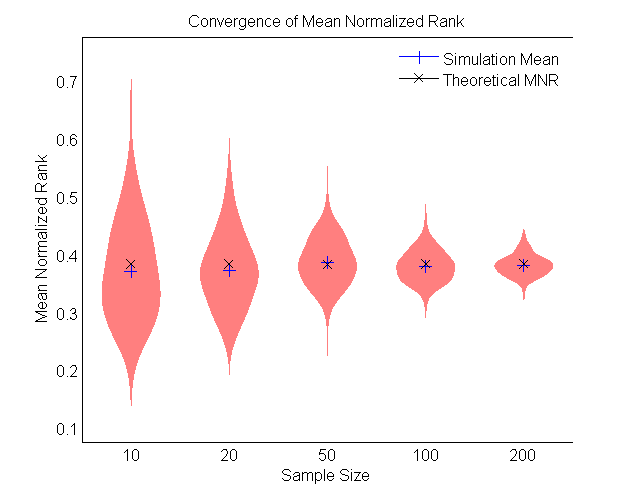
\includegraphics[width=4in]{simumnr_violin}
\end{center}
\caption{Simulation results}
\end{figure*}

\subsection{Simulation Experiment: Comparing MNR and I2C2}
\noindent In this subsection, we use simulated data to demonstrate the utility of MNR. In addition, comparison is made between MNR and another discriminability measure I2C2. I2C2 is another discriminability measure introduced in paper (**). Under additive noise assumption, I2C2 is defined to be one minus the ratio of within subject variance over total variance. That is given $O_{ij}=X_i+Z_{ij}$,
 
\[ I2C2=1-\frac{\text{Trace}(\text{Cov}(Z_{ij}))}{\text{Trace}(\text{Cov}(O_{ij}))} \]

In practice, $\text{Cov}(Z_{ij})$ and $\text{Cov}(O_{ij})$ need to be estimated from data. Compared to I2C2, MNR has a few advantages. First, MNR is a more generalized and non-parametric measure of discriminability. MNR can be easily extended to non-Euclidean metric and still be able to interpreted as a probability. Due to the fact that MNR rely on fewer assumptions and only estimate the probability, it turns out that relative standard error of MNR estimate is usually less than I2C2. Furthermore, non-additive noise and non-continuous data cannot be properly handled by I2C2. Even in continuous and additive noise setting, I2C2 is only determined by first two moments of data and is not sensitive to higher moments or correlations between noises.\\
\\
In the coming experiment, we consider four data generation scheme. We assume there are only two subjects under study, and $50$ observations in $\mathbb{R}^2$ are generated for each subject. Then we compute ICC of the first dimension, ICC of the second dimension, I2C2 and MNR. For each data generation scheme, $100$ repetitions are done. The figure 2 shows the result.\\
\\
\textbf{Scheme 1:} The noise is additive independent multivariate normal distribution. That is $O_{ij}=X_i+Z_{ij}$, where $X_1=[1,1]$, $X_2=[1,-1]$ and $Z_{ij}\sim\text{MVN}(0,(\begin{matrix} 1 & 0 \\ 0 & 2\end{matrix}))$. \\
\textbf{Scheme 2:} The data is generately essentially the same as scheme 1, but rotated $\frac{\pi}{4}$. That is $O_{ij}=X_i+Z_{ij}$, where $X_1=[\sqrt{2},0]$, $X_2=[0,-\sqrt{2}]$, $Z_{ij}\sim\text{MVN}(0,(\begin{matrix} 1.5 & 0.5 \\ 0.5 & 1.5\end{matrix}))$. \\
\textbf{Scheme 3:} The noise is still additive but generated from Laplacian distribution. That is $O_{ij}=X_i+Z_{ij}$, where $X_1=[1,1]$, $X_2=[1,-1]$. The first dimension of $Z_{ij}$ is generated from $\text{Laplace}(0,\frac{1}{\sqrt{2}})$, and the second dimension is generated from $\text{Laplace}(0,1)$. The parameters are chosen to make sure two subject conditional distributions has the same mean and covariance matrix as in scheme 1. \\
\textbf{Scheme 4:} The noise is multiplicative generated from log-normal distribution. That is $O_{ij}=X_i*Z_{ij}$, where $X_1=[1,1]$, $X_2=[1,-1]$  and $Z_{ij}\sim\text{LN}([\ln{2},\ln{3}],(\begin{matrix} \ln{2} & 0 \\ 0 & \ln{3}\end{matrix}))$. The parameters are chosen to make sure two subject conditional distributions has the same mean and covariance matrix as in scheme 1. \\
\begin{figure*}[t!]
\begin{center}
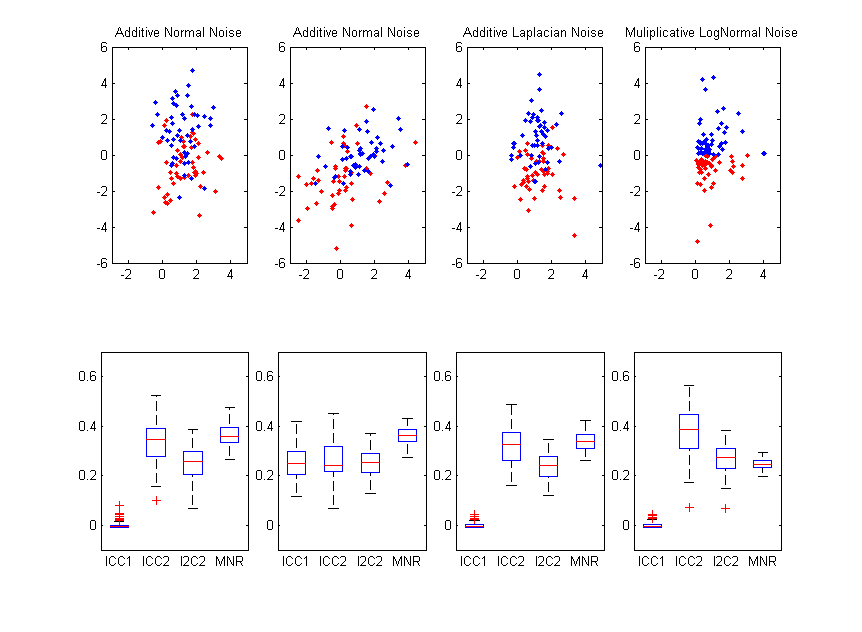
\includegraphics[width=5in]{Simu1}
\end{center}
\caption{Simulation results}
\end{figure*}

\noindent In figure 1, the scatter plots at the top are observations from two subjects, and the box plots at the bottom are the corresponding discriminability measures. First, it is not surprising that one dimensional discriminability measure ICC does not capture discriminability of higher dimensional data. Comaring scheme 1 and scheme 2, we expect that simple rotation does not affect discriminability; however, ICCs of two dimensions change substantially. Second, we can see I2C2 does not fully reflect the discriminability of data. In all four cases, I2C2 are roughly the same due to the fact we fix the first and second moments of data. However, we can see from the scatter plots that observations of scheme 3 is slightly more separated than observations of scheme 1, and observations of scheme 4 is mostly separated. At last, I2C2 clearly has larger estimation variance than MNR. This is partly due to the fact that I2C2 have more parameters to estimate. In order to compute I2C2, we must first estimate diagonal terms of two covariance matrices which leads to large variance in I2C2 estimate.   \\
\\
In this simple setting, we can quantify the degree of separation between two subjects by using Bayes error. Two subjects can be treated as two classes, and the Bayes errors of four schemes are $0.2395$, $0.2395$, $0.1839$ and $0$ respectively. It can be seen that MNR respects this ordering and reflects the degree of separation between subjects.   If we are interested in predicting a phenotype, our intuition is that the error rate will more likely to be small, when there is more separation between subjects. We conclude here that MNR is a better discriminability measure.


\subsection{Simulation Experiment: Maximizing Discriminability}
\noindent In this experiment, we demonstrate discriminability can be used to select parameter in data preprocessing. As in the last section, we consider only 2 subjects, each with s observations in $\mathbb{R}^2$. Again, we consider additve noise setting. The means of two subjects are $X_1=[1,0]$ and $X_2=[-1,0]$ respectively. For the noise, we consider two cases. The first case is $Z_{ij}\sim\text{MVN}([0,0],(\begin{matrix} 4 & 0 \\ 0 & 1\end{matrix}))$ and the second case is $Z_{ij}\sim\text{MVN}([0,0],(\begin{matrix} 1 & 0 \\ 0 & 4\end{matrix}))$. \\
\\
Now, assuming we want to linearly project the observations into 1 dimensional space. To achieve this, we sample possible lines to project uniformly from sphere, and compute discriminability of projection. Then, we choose the projection which has maximum MNR. Also, PCA is performed for comparison. Because of the way that data is generated, we see the optimal linear projection should be projecting observations onto x-axis, and Bayes error is the same before and after this projection. The figure 3 shows the result. From the figure, we see both MNR PCA give the optimal projection in the first case. However, in the second case only MNR gives the optimal projection. In this case, the second dimension has larger variance than the first dimension; therefore, PCA choose y-axis to project to.

\begin{figure*}[t!]
\begin{center}
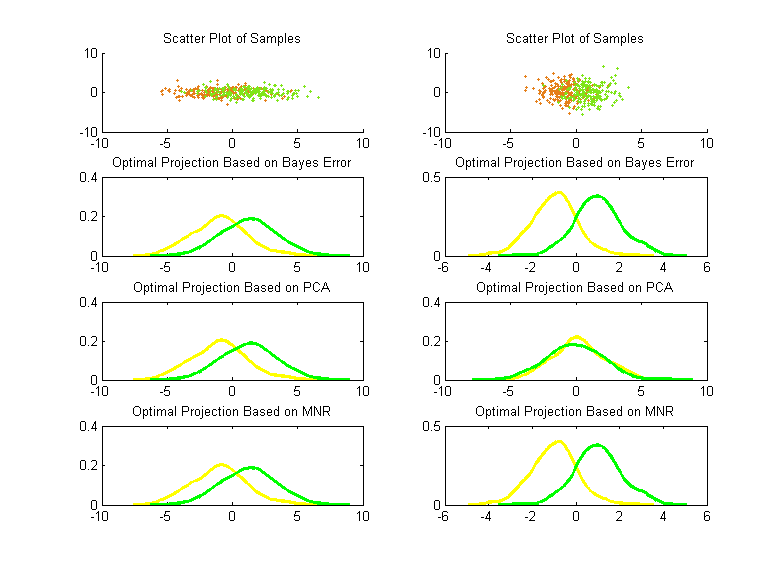
\includegraphics[width=4in]{parameter_selection_2sub}
\end{center}
\caption{Simulation results}
\end{figure*}


\section{Real Data Experiment}
\subsection{Human Connectome Data: NKI}
The first real data set analyzed is a human connectome data set NKI. There are $176$ subjects in the data set and each subject's brain is scanned twice ($n=176$, $s=2$). The original time series data is parcellized and the brain is divided into $131$ and $165$ regions. We first compute a correlation matrix which record correlations between different regions of the brain. The correlation matrix is then thresholded by $t$. Specifically, there is an edge between two regions if and only if the absolute correlation between two regions are greater than $t$. In this way, we construct a graph from each brain scan.\\ 
\\
Despite brain scans, demographic information including age and gender of subjects is also collected. The inference task is to predict age and gender of a subject based on the graph derived from his or her brain scan. K-Nearest Neighbor rule is applied to predict both age and gender. In this experiment, we are interested in how to correctly select the threshold $t$ and how the threshold affects inference results. Figure 4 and 5 summarize the results.\\



\noindent From figure 4 and 5, we can see the processed data is most discriminable when the threshold $t$ is around $0.16$. Meanwhile, mean squared error of age prediction and classification error of gender prediction are also close to their minimums. Gender and age are two uncorrelated variables in the data set. Therefore, this experiment demonstrates that processed data of maximum discriminability is optimal for two independent inference tasks. 

\subsection{Human Connectome Data: HCP}
HCP is another human connectome data set we analyze. In the data set, 476 subjects are each scanned 4 times. Scans are then parcellized into 25, 50, 100, 200 and 300 regions. Again we compute the correlation matrix and threshold it to construct a graph for each brain scan. Age and gender are then predicted based on the constructed graph.\\


\noindent Figure 6-10 show similar results. The most discriminable processed data has smallest classification error. However, mean square error of age prediction seems to just fluctuate randomly. This may due to the fact that age prediction is a much harder task and the K-NN is not good enough to capture the change of differentiability of processed data.\\
\\
A natural question to ask next is that among these 7 connectome data sets which one is most discriminable. The question can be answered by comparing MNR. For each data set, we first choose the threshold $t$ which maximizes discriminability and then compare the corresponding MNR across data set. A standard error estimate is also calculated by assuming normalized ranks are independent. The assumption leads to underestimate the standard error due to mild positive correlations between normalized ranks. To test whether two data sets are of same discriminability, we can construct to confidence intervals of MNR and check whether they overlap or not. \\
\\
Table 1 below summarizes the results. Two NKI data sets are remarkably more discriminable compared to 5 HCP data sets. Discriminability of NKI131 tends to be better than discriminability of NKI165, but the difference is not statistical significant. Among 5 HCP data sets, HCP100 tends to be the most discriminable one. By looking at HCP data sets alone, we discover another interesting fact that discriminability demonstrates some kinds of bias-variance tradeoff. When the brain is partitioned into very few regions, the data set is not discriminable possibly due to large bias. When the brain is partitioned into a large number of regions, the data set is also not discriminable due to large variance. 

\begin{table}

\begin{center}
  \begin{tabular}{| p{2.5 cm} | p{2.5 cm} | p{2.5 cm} |}
    \hline
    Data Set & Mean Rank & S.E. \\ \hline
    NKI131 & 0.0151 & 0.0034 \\ \hline
    NKI165 & 0.0215 & 0.0044 \\ \hline
    HCP25 & 0.1393 & 0.0030 \\ \hline
    HCP50 & 0.1077 & 0.0029 \\ \hline
    HCP100 & 0.0753 & 0.0024 \\ \hline
    HCP200 & 0.0843 & 0.0026 \\ \hline
    HCP300 & 0.0944 & 0.0027 \\ \hline
%    \hline
  \end{tabular}
  \caption{Discriminability Comparison}
\end{center}
\end{table}




\section{Conclusion}
In the sections above, we demonstrate that maximizing discriminability helps improving prediction accuracy. Our work provides guidance and direction to scientists on data preprocessing. Particularly, when facing decisions which are hard to make in data preprocessing, scientists should consider preprocessing method which maximizes discriminability of processed data.\\
\\
The current work can be extended in both theoretical and practical directions. From theoretical aspect, we only show Bayes error rate varies with discriminability. It is also interesting to see the classification error of a specific classifier varies with discriminability. Secondly, assumptions of theoretical analysis should be relaxed. Assumptions include additive noise, independence between noise and true values, and Euclidean distance maybe relaxed to better model real data. Thirdly, we only analyze the relationship between classification and discriminability. More inference tasks should be considered. These inference tasks can be but not limit to hypothesis testing, regression and clustering. Their relationship to discriminability should be investigated.\\
\\ 
From the aspect of practice, the whole data preprocessing procedure should be studied. In the experiments above, we focus on only one step of the data preprocessing. We may investigate discriminability of data preprocessing step as a whole or even starting at data collection step. Secondly, more data experiments should be done in different setting to prove utility of discriminability in data preprocessing. Data of more complicated form or with non-Euclidean distance can be investigated in a similar manner. The points mentioned in this and last paragraph can all extend our current work and improve its applicability. Nevertheless, our primary purpose is to demonstrate the relationship between discriminability and predictability.



\section{Other Stuff}


Consider the following generative process.  For each sample $i$, there exists some true physical property $\bv_i$.  In our running example throughout this article, $\bv_i$ is the true connectome of subject $i$.
Unfortunately, we do not get to directly observed $\bv_i$, rather, we measure it with some device, that transforms the truth from $\bv_i$ to $\bw_i$ via $f_{\bphi}$.  The parameter $\bphi \in \bPhi$ characterizes all options in the measurement, including, for example, which scanner to use, which resolution, the number of images, sampling rate, etc.  The output of $f_{\bphi}$ is the  ``raw'' observation data $\bw_i$, but it is corrupt in various ways, including movement or intensity artifacts introduced by the measurement process.  Therefore, rather than operating directly on $\bw_i$, we intentionally ``pre-process'' the data, in an effort to remove a number of nuisance variables.  This pre-processing procedure further transforms the data from $\bw_i$ to $\bx_i$ via $g_{\bpsi}$.   The parameter $\bpsi \in \bPsi$ indexes all pre-processing options, including whether to perform motion correction, which motion correction, deconvolution, etc.  More specifically, the entire code base, including dependencies, and even the hardware the pre-processing is running on, could count as $\bpsi$. For brevity,  we  define $\bx_i:= g_{\bpsi} \big(f_{\bphi} (\bv_i) \big)$.

In addition to $\bv_i$, there are other properties of sample $i$ of interest; we call all of them $\by_i \in \mc{Y}$.  These may include, for example, the phenotype of the subject, including personality tests, demographic information, and genetic data.  The goal of experimental design, in this context, is to choose $\bphi \in \bPhi$ and $\bpsi \in \bPsi$ to maximize some function of  $(\bx_i, \by_i)$.  



To quantify the performance of our choice, we introduce some assumptions.  First, assume that each $(\bV_i,\bY_i)$ pair is sampled independently and identically from some distribution, $(\bV_i,\bY_i) \iid F_{V,Y}$.  For simplicity, let us assume that our goal is regression, using $\bX_i$ as the \emph{predictor} variables, and a single dimension of $\bY_i$ as the \emph{target} variable (we will generalize these assumptions below).  Moreover, let $h \from \mc{X} \to \mc{Y}$ be the regression function (which we will typically learn from the data).  The loss function, $\ell$ quantifies the error of our predictions, $\ell( h(\bx_i), \by_i) \in \Real_+$.  
% Moreover, we assume that there exists some desired action, $\mb{a}_i^* \in \mc{A}$, and a loss function, $\ell: h(\mc{X},\mc{Y}) \times \mc{A} \to \Real_+$ that evaluates the performance of our function.  For example, $h(\cdot)$ might be a regression function that operates only on $\mc{X}$, in which case the loss might be squared error distance between the predicted value of $\bY_i$ and its true value.  
In the above described scenario, we can characterize our desiderata as minimizing the risk, or expected loss, under the above assumptions:
\begin{equation} \label{eq:goal}
\begin{aligned}
& \underset{\bphi \in \bPhi,\bpsi \in \bPsi}{\text{minimize}}
& & \EE [ \ell( h (\bx_i), \by_i)],
\end{aligned}
\end{equation}
where the expectation is taken with respect to the joint distribution of $X$ and $Y$, which is induced by the joint distribution of $(\bV,\bY)$, and transformed by $f(\cdot)$ and $g(\cdot)$; that is, $F_{X,Y}:=F_{f(g(V),Y}$.

Problem \eqref{eq:goal} is an experimental design question.  However, in the scenario of interest, $\by$ is not observed.  Therefore, we cannot directly optimize Problem \eqref{eq:goal}, and instead, we must consider some surrogate function.  


We propose to borrow an idea from generalizability theory (or G theory), in particular, by introducing ``facets''.  A facet is a particular source of variance.  For simplicity, consider the following illustrative scenario (we will generalize this idea below). In particular, assume that our goal is to optimize the pre-processing routine, encoded by $\bpsi$. Let $i$ denote the sample's unique \emph{identity} (hereafter, referred to as the \emph{subject}) and $t$ denote the trial number.  Thus, there is a single $\bv_i$ for subject $i$, but we have $\bw_{i,t}$, which is the $t^{th}$ trial, implicitly also a function of $\bphi$, which encodes all the details of the measurement.  If both $f$ and $g$ together do not introduce too much noise, then we would expect that $\bx_{i,1}$ and $\bx_{i,2}$ are \emph{closer} to one another than either are to any other subject's data, $\bx_{i',t}$.  Define $\delta$ to be a metric computing the distance between two data points, $\delta \from \mc{X} \times \mc{X} \to \Real_+$.  Formally, we expect that $\delta(\bx_{i,t},\bx_{i,t'}) \leq \delta(\bx_{i,t},\bx_{i',t''})$, for any $i,i',t,t',t''$.  
For brevity, let $\delta_{i,t,t'}:=\delta(\bx_{i,t}, \bx_{i,t'})$ and 
$\delta_{i,i',t,t'}:=\delta(\bx_{i,t}, \bx_{i',t''}$.  
This intuition leads to our definition of discriminability:
\begin{align}
R(\bpsi,\bphi,F) = \PP[ \delta_{i,t,t'} \leq \delta_{i,i',t,t'}]
\end{align}


Now, we can consider a surrogate objective function:
\begin{equation} \label{eq:surroage}
\begin{aligned}
& \underset{\bpsi \in \bPsi}{\text{minimize}}
& & \EE [ \ell( \bx_{i,1}, \bx_{i,2})],
\end{aligned}
\end{equation}

% \appendices
\section{Proof of Lemmas}
%\subsubsection*{Proof for Lemma 1}
\begin{proof}[Proof of Lemma 1]
By definition of $R$,
\[E(R)= \frac{\sum\limits_{i=1}^{n} \sum\limits_{j=1}^{s}  \sum\limits_{k=1,k\neq j}^{s} E(R_{ijk})}{ns(s-1)}\]
The expectation of $R_{ijk}$ can be simplified,
\begin{eqnarray*}  
& &E(R_{ijk}) \\
&=&\frac{\sum\limits_{p=1,p\neq i}^{n} \sum\limits_{q=1}^{s} E(I\{\|O_{ij}-O_{pq}\| < \|O_{ij}-O_{ik}\| \}) }{(n-1)s} \\
&=&\frac{\sum\limits_{p=1,p\neq i}^{n} \sum\limits_{q=1}^{s} P(\|O_{ij}-O_{pq}\| < \|O_{ij}-O_{ik}\| ) }{(n-1)s} \\
&=&P(\|O_{ij}-O_{pq}\| < \|O_{ij}-O_{ik}\|) \text{ for any $p\neq i$}
\end{eqnarray*}
The last equality is due to the fact that $O$s have the same distribution. Notice the symmetry of $R_{ijk}$ in $i$, $j$ and $k$ we have,
\[E(R)=E(R_{ijk})=P(\|O_{ij}-O_{pq}\| < \|O_{ij}-O_{ik}\|)\]
\end{proof}

\begin{proof}[Proof of Lemma 2]
By definition of $R$,
\begin{eqnarray*}  
R &=&\frac{\sum\limits_{i,j,k,k\neq j} R_{ijk}}{ns(s-1)}\\
&=& \frac{\sum\limits_{i,j,k,k \neq j,p,p\neq i,q} I_{ijkpq}}{ns(s-1)(n-1)s}\\
\end{eqnarray*}
Here, $I_{ijkpq}:=I\{\|O_{ij}-O_{pq}\| < \|O_{ij}-O_{ik}\| \}$. We show in the previous lemma that $E(R)=P(\|O_{ij}-O_{pq}\| < \|O_{ij}-O_{ik}\|)$. To demonstrate that $R$ converges to its epxectation in probability, it is suffice to show that $\text{Var}(R) \rightarrow 0$. Since then, by Chebyshev's inequality,
\[P(|R-E(R)| \geq \epsilon) \leq \frac{\text{Var}(R)}{\epsilon^2} \rightarrow 0\]
If we expand the variance of $R$, 
\[\text{Var}(R)= \frac{\sum\limits_{i,j,k,p,q} \sum\limits_{i',j',k',p',q'} \text{Cov}(I_{ijkpq},I_{i'j'k'p'q'})}{(ns(s-1)(n-1)s)^2} \]
There are $(ns(s-1)(n-1)s)^2$ terms in the sum at the nominator; however, some of them are actually 0. $I_{ijkpq}$ is a function of $O_{ij}$, $O_{ik}$ and $O_{pq}$; therefore, is independent of any observations of subjects other than $i$ and $p$. This implies $I_{ijkpq}$ is independent of $I_{i'j'k'p'q'}$ as long as $\{i,p\} \cap \{i',p'\} = \emptyset$. As a consqeunce, there are $(4n-6)(s(s-1)s)2=ns(s-1)(n-1)s-(n-2)s(s-1)(n-3)s$ combinations of $i'j'k'p'q'$ such that covariance between $I_{ijkpq}$ and $I_{i'j'k'p'q'}$ maybe non-zero. Furthermore, the covariance must be less $\frac{1}{4}$ due to the fact that they are indicator random variables. Therefore, we have 
\begin{eqnarray*} 
\text{Var}(R)&=& \frac{\sum\limits_{i,j,k,p,q} \sum\limits_{i',j',k',p',q'} \text{Cov}(I_{ijkpq},I_{i'j'k'p'q'})}{(ns(s-1)(n-1)s)^2} \\
&\leq& \frac{\sum\limits_{i,j,k,p,q}  (4n-6)(s(s-1)s)}{4(ns(s-1)(n-1)s)^2} \\
&=& \frac{ (ns(s-1)(n-1)s)(4n-6)(s(s-1)s)}{4(ns(s-1)(n-1)s)^2} \\
&=& \frac{(4n-6)}{4n(n-1)} \\
&\leq& \frac{1}{n}  \\
&\rightarrow& 0 \text{ , as $n\rightarrow \infty$} 
\end{eqnarray*}
As discussed above, this concludes the proof for the lemma.
\end{proof}

\begin{proof}[Proof of Lemma 3]
By Lemma 1, we only need to bound $P(\|O_{ij}-O_{ik}\| < \|O_{ij}-O_{pq}\|)$. Under additive noise setting,
\begin{eqnarray*}
& &P(\|O_{ij}-O_{ik}\| < \|O_{ij}-O_{pq}\|) \\
&=&P(\|Z_{ij}-Z_{ik}\| < \|X_{i}+Z_{ij}-X_{p}-Z_{pq}\|) \\
&\geq&P(\|Z_{ij}-Z_{ik}\| < \|X_{i}-X_{p}\| - \|Z_{ij}-Z_{pq}\|) \\
&=& P(\|Z_{ij}-Z_{ik}\|+\|Z_{ij}-Z_{pq}\|< \|X_{i}-X_{p}\|) \\
&\geq& P(\|Z_{ij}-Z_{ik}\|^2+\|Z_{ij}-Z_{pq}\|^2< \|X_{i}-X_{p}\|^2) \\
\end{eqnarray*}
To bound the probability above, we bound the two terms on different sides of equation separately. We start with the term at the left side and compute its expectation.
 \begin{eqnarray*}
 & &E(\|Z_{ij}-Z_{ik}\|^2+\|Z_{ij}-Z_{pq}\|^2) \\
 &=&2 E(\|Z_{ij}-Z_{ik}\|^2) \\
 &=&2 E(Z_{ij}^T Z_{ij}+Z_{ik}^T Z_{ik} +2Z_{ij}^T Z_{ik}) \\
 &=&4\sigma_1^2
 \end{eqnarray*}
 We then use Markov's Inequality to this term, 
 \[P(\|Z_{ij}-Z_{ik}\|^2+\|Z_{ij}-Z_{pq}\|^2 < k\sigma_1^2) \geq 1-\frac{4}{k} \]
 Similarly, we compute the expectation of second term.
  \begin{eqnarray*}
  & &E(\|X_{i}-X_{p}\|^2) \\
  &=&E(X_{i}^T X_{i}+X_{p}^T X_{p}+2X_{i}^T X_{p}) \\
  &=&2\sigma_2^2 \\
  &=&2\lambda^2\sigma_1^2
  \end{eqnarray*}
Then, we apply Paley-Zygmund Inequality,
\[P(\|X_i-X_p\|^2 > k\sigma_1^2 ) \geq c(1-\frac{k}{2\lambda^2})^2 \]
Understand the fact that $X$s and $Z$s are independent, we can combine the two inequalities and get a bound on $P(\|O_{ij}-O_{ik}\| < \|O_{ij}-O_{pq}\|)$.
\begin{eqnarray*}
& &P(\|O_{ij}-O_{ik}\| < \|O_{ij}-O_{pq}\|) \\
&\geq& P(\|Z_{ij}-Z_{ik}\|^2+\|Z_{ij}-Z_{pq}\|^2< \|X_{i}-X_{p}\|^2) \\
&\geq& P(\|Z_{ij}-Z_{ik}\|^2+\|Z_{ij}-Z_{pq}\|^2<k\sigma_1^2) \\
& & \times P(\|X_i-X_p\|^2 > k\sigma_1^2 ) \\
&\geq& c(1-\frac{k}{2\lambda^2})^2(1-\frac{4}{k}) \\
&=&c(1-\frac{\sqrt{2}}{\lambda})^3
\end{eqnarray*}
The last equality is the result by setting $k=2\sqrt{2}\lambda$. This leads to the final result on the expectation of mean normalized rank.
\begin{eqnarray*}
E(R)&=&1-P(\|O_{ij}-O_{ik}\| < \|O_{ij}-O_{pq}\|) \\
&\leq& 1-c(1-\frac{\sqrt{2}}{\lambda})^3
\end{eqnarray*}
We can also solve for and lower bound $\lambda$.
\[\lambda \geq \frac{2^{\frac{1}{4}}}{1-(\frac{1-E(R)}{c})^{\frac{1}{3}}} \]
\end{proof}


\begin{proof}[Proof of Lemma 4]
To compute Mahalanobis distance, we first compute weighted covariance matrix.
\begin{eqnarray*}
\text{Var}(O|Y=i) &=& \text{Var}(X|Y=i)+\text{Var}(Z|Y=i) \\
&=& \Sigma_i+\frac{1}{\lambda^2}\Sigma
\end{eqnarray*}
Therefore, the weighted covariance matrix of $O$s
\begin{eqnarray*}
\Sigma_\lambda&=&\pi_0\text{Var}(O|Y=0)+\pi_1\text{Var}(O|Y=1) \\
&=&\pi_0\Sigma_0+\pi_1\Sigma_1+\frac{1}{\lambda^2}\Sigma
\end{eqnarray*}
Then, apply Devijver and Kittler's result,
\[L_\lambda \leq \frac{2\pi_0\pi_1}{1+\pi_0\pi_1(\mu_0-\mu_1)^T\Sigma_\lambda^{-1}(\mu_0-\mu_1)}\]
\end{proof}

% you can choose not to have a title for an appendix
% if you want by leaving the argument blank




\newpage
\small{
\bibliography{biblio}
\bibliographystyle{IEEEtran}
}


\end{document}
